\section{Results}

\subsection{In-domain pragmatic performance}
Table~\ref{tab:q1a} reports six pragmatic binary macro-F1 metrics as mean $\pm$ sample SD over three runs for trainable rows. Among the evaluated systems with complete three-run results, XLM-R-large multi-task (ours) has the highest observed mean on all six pragmatic heads and on macro-pragmatic F1. Against the XLM-R-large pragmatic-only baseline, the proposed system has higher observed means on all six pragmatic heads: +0.41 pp for implicit sentiment, +0.96 pp for sarcasm, +0.25 pp for irony, +0.76 pp for idiom/figurative language, +0.50 pp for code-switching, and +0.89 pp for mocking. At the aggregate level, the difference computed from the unrounded three-run scores is +0.63 pp. The paired hierarchical bootstrap gives a nominal 95\% CI of [+0.07,+1.20] pp for this aggregate difference. All six individual head-level intervals cross zero, so the per-head gains are treated as descriptive rather than as head-specific significance claims.

\begin{table*}[tb]
\centering
\small
\setlength{\tabcolsep}{0pt}
\begin{tabularx}{\textwidth}{>{\raggedright\arraybackslash}p{0.90in} @{\hspace{1.5pt}} >{\centering\arraybackslash}p{0.75in} @{\hspace{1.5pt}} >{\centering\arraybackslash}p{0.75in} @{\hspace{1.5pt}} >{\centering\arraybackslash}p{0.75in} @{\hspace{1.5pt}} >{\centering\arraybackslash}p{0.75in} @{\hspace{1.5pt}} >{\centering\arraybackslash}p{0.75in} @{\hspace{1.5pt}} >{\centering\arraybackslash}p{0.75in} @{\hspace{1.5pt}} >{\centering\arraybackslash}p{0.75in}}
\hline
Model & Implicit & Sarcasm & Irony & Idiom & Code-sw. & Mocking & Macro-F1 \\
\hline
\shortstack[l]{\textbf{XLM-R-large}\\\textbf{MT (ours)}} & \mbox{\textbf{92.67} $\pm$ 0.24} & \mbox{\textbf{89.36} $\pm$ 0.90} & \mbox{\textbf{98.43} $\pm$ 0.20} & \mbox{\textbf{93.35} $\pm$ 0.66} & \mbox{\textbf{94.84} $\pm$ 0.56} & \mbox{\textbf{93.35} $\pm$ 0.73} & \mbox{\textbf{93.67} $\pm$ 0.19} \\
PhoBERT ST & \mbox{88.00 $\pm$ 1.29} & \mbox{70.87 $\pm$ 1.34} & \mbox{97.13 $\pm$ 1.06} & \mbox{91.21 $\pm$ 0.78} & \mbox{91.08 $\pm$ 1.51} & \mbox{79.16 $\pm$ 2.99} & \mbox{86.24 $\pm$ 0.49} \\
PhoBERT fine-tune & \mbox{85.76 $\pm$ 0.72} & \mbox{72.64 $\pm$ 0.50} & \mbox{97.45 $\pm$ 0.19} & \mbox{86.63 $\pm$ 0.66} & \mbox{91.73 $\pm$ 0.53} & \mbox{78.53 $\pm$ 1.01} & \mbox{85.46 $\pm$ 0.36} \\
\shortstack[l]{XLM-R-large\\pragmatic-only} & \mbox{92.25 $\pm$ 0.10} & \mbox{88.40 $\pm$ 0.36} & \mbox{98.18 $\pm$ 0.21} & \mbox{92.59 $\pm$ 0.39} & \mbox{94.34 $\pm$ 0.19} & \mbox{92.45 $\pm$ 0.52} & \mbox{93.04 $\pm$ 0.04} \\
Sailor-7B SFT & \mbox{85.42 $\pm$ 0.27} & \mbox{72.14 $\pm$ 2.96} & \mbox{95.75 $\pm$ 0.52} & \mbox{91.15 $\pm$ 1.40} & \mbox{91.03 $\pm$ 0.74} & \mbox{77.76 $\pm$ 1.21} & \mbox{85.54 $\pm$ 0.48} \\
Vistral-7B SFT & \mbox{87.36 $\pm$ 0.31} & \mbox{74.74 $\pm$ 0.94} & \mbox{96.69 $\pm$ 0.23} & \mbox{91.48 $\pm$ 1.55} & \mbox{92.80 $\pm$ 0.60} & \mbox{79.91 $\pm$ 0.26} & \mbox{87.16 $\pm$ 0.33} \\
\shortstack[l]{GPT-4.1-mini\\zero-shot} & 45.44 & 56.51 & 53.17 & 52.45 & 62.42 & 54.69 & 54.11 \\
\shortstack[l]{GPT-4.1-mini\\8-shot} & 49.04 & 61.09 & 52.37 & 50.87 & 56.89 & 54.32 & 54.10 \\
\hline
\end{tabularx}
\caption{Q1a pragmatic binary macro-F1. Trainable systems report mean $\pm$ sample SD over three runs; GPT-4.1-mini rows are single-run references. MT = multi-task; ST = single-task. The XLM-R-large pragmatic-only baseline uses the same Q1a training and model-selection settings as the proposed model but optimizes only the six pragmatic tasks. Bold means mark the proposed model.}
\label{tab:q1a}
\end{table*}

\subsection{External affective transfer}
Table~\ref{tab:secondary}(a) reports external macro-F1 values, with Mean defined as the unweighted mean across UIT-VSFC, UIT-VSMEC, and AIVIVN. XLM-R-large multi-task (ours) is 1.2, 0.2, and 0.4 pp below XLM-R-large 8-head baseline on UIT-VSFC, UIT-VSMEC, and AIVIVN, respectively. Its mean external macro-F1 is 42.0 versus 42.5 for XLM-R-large 8-head baseline, 41.3 for Sailor, and 39.7 for Vistral.

\begin{table*}[t]
\centering
\begin{minipage}[t]{0.49\textwidth}
\centering
\textbf{(a) Q1b external affective transfer}
\par\smallskip
\footnotesize
\setlength{\tabcolsep}{1.5pt}
\begin{tabularx}{\linewidth}{>{\raggedright\arraybackslash}p{0.60in} >{\centering\arraybackslash}X >{\centering\arraybackslash}X >{\centering\arraybackslash}X >{\centering\arraybackslash}X}
\hline
Model & VSFC & VSMEC & AIVIVN & Mean \\
\hline
\shortstack[l]{PhoBERT\\ST} & \mbox{29.7\,$\pm$\,0.5} & \mbox{38.8\,$\pm$\,1.5} & \mbox{45.4\,$\pm$\,2.6} & \mbox{38.0\,$\pm$\,0.3} \\
\shortstack[l]{PhoBERT\\MT} & \mbox{33.6\,$\pm$\,3.0} & \mbox{36.4\,$\pm$\,0.7} & \mbox{44.7\,$\pm$\,1.3} & \mbox{38.2\,$\pm$\,1.5} \\
\shortstack[l]{XLM-R\\8H} & \mbox{39.1\,$\pm$\,1.1} & \mbox{40.2\,$\pm$\,0.2} & \mbox{48.3\,$\pm$\,1.2} & \mbox{42.5\,$\pm$\,0.5} \\
\shortstack[l]{XLM-R\\MT (ours)} & \mbox{37.9\,$\pm$\,2.8} & \mbox{40.0\,$\pm$\,0.7} & \mbox{47.9\,$\pm$\,2.2} & \mbox{42.0\,$\pm$\,1.8} \\
\shortstack[l]{Sailor-7B} & \mbox{34.4\,$\pm$\,3.2} & \mbox{40.7\,$\pm$\,0.7} & \mbox{48.7\,$\pm$\,1.4} & \mbox{41.3\,$\pm$\,1.2} \\
\shortstack[l]{Vistral-7B} & \mbox{30.7\,$\pm$\,6.4} & \mbox{39.4\,$\pm$\,1.5} & \mbox{49.0\,$\pm$\,0.8} & \mbox{39.7\,$\pm$\,2.5} \\
\hline
\end{tabularx}
\end{minipage}
\hfill
\begin{minipage}[t]{0.49\textwidth}
\centering
\textbf{(b) Q2 ablations}
\par\smallskip
\small
\setlength{\tabcolsep}{0pt}
\begin{tabularx}{\linewidth}{>{\raggedright\arraybackslash}p{0.78in} >{\centering\arraybackslash}X >{\centering\arraybackslash}X >{\centering\arraybackslash}X}
\hline
Variant & Prag. F1 & \shortstack[c]{Polarity ECE\\$\times 10^3$ $\downarrow$} & Rel. GPU-h \\
\hline
Full & 92.8 $\pm$ 0.6 & 81.1 $\pm$ 11.7 & 1.00 \\
$-$ Emotion & 91.7 $\pm$ 0.7 & 56.2 $\pm$ 22.5 & 0.65 \\
$-$ Rationale & 92.3 $\pm$ 1.3 & 68.1 $\pm$ 22.2 & 0.20 \\
\shortstack[l]{No multi-task\\sharing$^\dagger$} & 74.7 $\pm$ 2.3 & 118.9 $\pm$ 69.1 & 1.10 \\
$-$ Polarity & 92.8 $\pm$ 0.2 & n/a & 0.81 \\
$-$ Uncertainty weighting & 92.9 $\pm$ 0.3 & 90.2 $\pm$ 5.9 & 0.82 \\
\hline
\end{tabularx}
\end{minipage}
\caption{Secondary analyses. (a) Q1b external macro-F1; Mean is the unweighted average over UIT-VSFC, UIT-VSMEC, and AIVIVN. ST = single-task; MT = multi-task; 8H = eight-head baseline. (b) Q2 ablations; ECE is polarity development ECE ($\times 10^3$), and GPU-h is normalized to the full Q2 XLM-R-large model. $\dagger$ Eight independently trained task-specific components.}
\label{tab:secondary}
\end{table*}

\subsection{Auxiliary-task and uncertainty ablations}
Table~\ref{tab:secondary}(b) is the separate Q2 follow-up cohort. Its training configuration uses a linear scheduler, a 0.10 warmup ratio, patience 2, and development macro-pragmatic F1 checkpoint selection. The full configuration reports $92.8 \pm 0.6$ F1, whereas removing task-uncertainty weighting reports $92.9 \pm 0.3$. The full model has lower reported ECE than the no-uncertainty variant, and the rationale-free configuration reduces relative cost. These are observed Q2 trade-offs; they do not imply that uncertainty weighting uniformly improves F1.


The no-sharing row aggregates eight single-task component outputs by sample ID. Q2 ECE is ten-bin top-label polarity development ECE on the $10^3$ scale, and cost is relative successful GPU-hours normalized to the full Q2 XLM-R-large model.

\subsection{Sarcasm performance under positive-label scarcity}
For Q3, the budgets constrain only positive sarcasm supervision. Each budget retains the full negative sarcasm pool, all other labels, and polarity and emotion supervision. Out-of-budget positives have only their sarcasm target and rationale loss masked; they remain available to the other task losses. The development and test splits remain fixed. Table~\ref{tab:q3} and Figure~\ref{fig:diagnostic-panels}(a) show the observed, non-monotonic curves.

\begin{figure*}[t]
\centering
\small
\setlength{\tabcolsep}{3pt}
\refstepcounter{table}
\begin{tabularx}{\textwidth}{>{\raggedright\arraybackslash}X >{\centering\arraybackslash}X >{\centering\arraybackslash}X >{\centering\arraybackslash}X}
\hline
\shortstack[c]{Positive sarcasm\\supervision budget} & \shortstack[c]{XLM-R-large\\multi-task (ours)\\sarcasm / macro} & \shortstack[c]{PhoBERT\\(fine-tune)\\sarcasm / macro} & \shortstack[c]{Vistral-7B SFT\\sarcasm / macro} \\
\hline
32 & 84.2 $\pm$ 1.6 / 91.1 $\pm$ 1.3 & 69.7 $\pm$ 1.5 / 84.2 $\pm$ 0.7 & 70.5 $\pm$ 2.4 / 86.2 $\pm$ 0.2 \\
64 & 83.7 $\pm$ 1.3 / 91.2 $\pm$ 0.8 & 70.8 $\pm$ 2.8 / 77.7 $\pm$ 11.8 & 72.5 $\pm$ 0.9 / 86.7 $\pm$ 0.5 \\
128 & 85.2 $\pm$ 0.7 / 91.6 $\pm$ 0.2 & 71.8 $\pm$ 2.2 / 84.0 $\pm$ 1.2 & 71.3 $\pm$ 0.6 / 86.2 $\pm$ 0.4 \\
256 & 85.3 $\pm$ 2.6 / 91.6 $\pm$ 1.2 & 73.4 $\pm$ 1.2 / 84.5 $\pm$ 0.9 & 64.0 $\pm$ 5.1 / 70.3 $\pm$ 14.2 \\
512 & 87.2 $\pm$ 1.2 / 92.3 $\pm$ 0.7 & 70.8 $\pm$ 2.8 / 78.1 $\pm$ 9.1 & 73.9 $\pm$ 1.2 / 87.2 $\pm$ 0.3 \\
Full & 85.0 $\pm$ 2.3 / 91.1 $\pm$ 1.3 & 73.3 $\pm$ 0.8 / 84.5 $\pm$ 0.1 & 75.3 $\pm$ 0.8 / 87.4 $\pm$ 0.2 \\
\hline
\end{tabularx}
\label{tab:q3}
\small\textbf{Table \thetable:} Q3 results under positive sarcasm supervision budgets; the first column is the positive sarcasm supervision budget, not the total training-set size.

\begin{minipage}{0.48\textwidth}
\centering
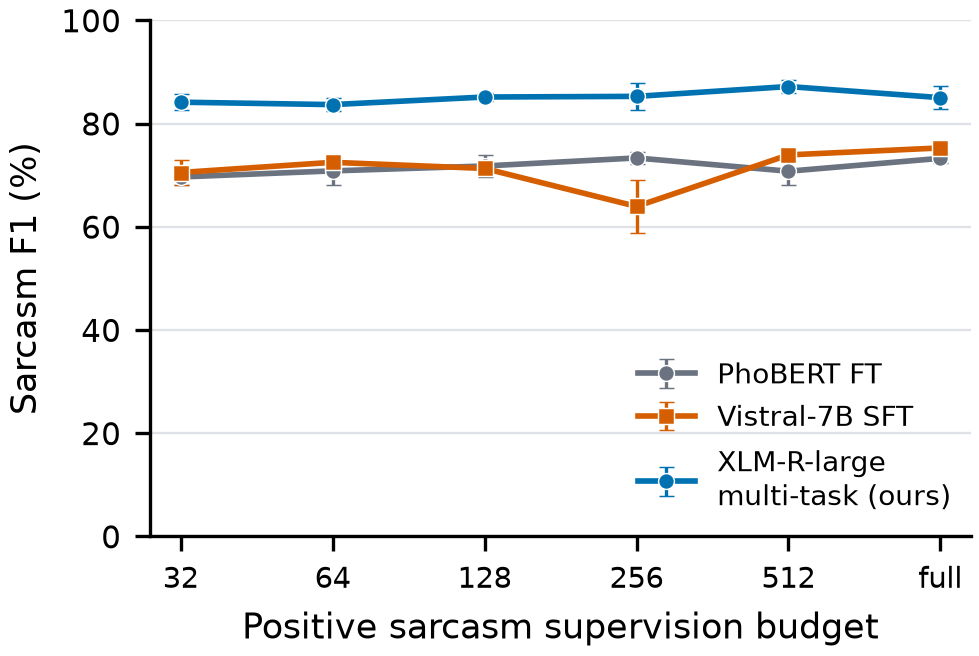
\includegraphics[width=\linewidth]{figures/figure_q3_sarcasm_budget.png}
\par\smallskip
\textbf{(a)}
\end{minipage}
\hfill
\begin{minipage}{0.48\textwidth}
\centering
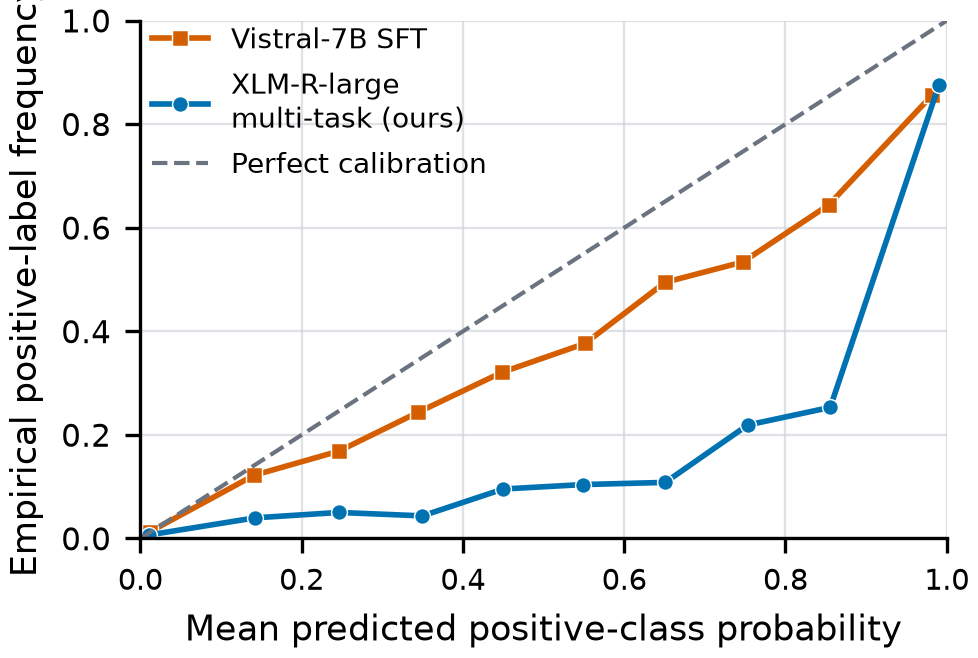
\includegraphics[width=\linewidth]{figures/figure_q4_reliability.png}
\par\smallskip
\textbf{(b)}
\end{minipage}
\refstepcounter{figure}
\label{fig:diagnostic-panels}
\par\smallskip
\small\textbf{Figure \thefigure:} Diagnostic analyses. (a) Sarcasm F1 under positive sarcasm supervision budgets. (b) Reliability diagrams for raw positive-class probabilities; points compare mean predicted probability with empirical positive-label frequency.
\end{figure*}

\subsection{Calibration}
Figure~\ref{fig:diagnostic-panels}(b) evaluates event calibration for the six pragmatic heads. It bins raw positive-class sigmoid probabilities and compares mean predicted positive-class probability with empirical positive-label frequency; no threshold is applied. XLM-R-large multi-task (ours) has ECE $0.0386 \pm 0.0069$, while Vistral has $0.0345 \pm 0.0041$. Since lower ECE is better, Vistral has the lower observed value; the numerical gap is small.
